\documentclass[runningheads]{llncs}

%\usepackage{subcaption}
%\captionsetup{compatibility=false}
\usepackage{authblk}
\usepackage{amsmath}
\usepackage{graphicx}
% \renewcommand\UrlFont{\color{blue}\rmfamily}
\usepackage{color}
\usepackage{listings}

\definecolor{gray}{rgb}{0.5,0.5,0.5}
\definecolor{mauve}{rgb}{0.58,0,0.82}

\lstset{ 
  language=SQL,                   % the language of the code
  basicstyle=\footnotesize,       % the size of the fonts that are used for the code
  numbers=left,                   % where to put the line-numbers
  numberstyle=\tiny\color{gray},  % the style that is used for the line-numbers
  stepnumber=1,                   % the step between two line-numbers. If it's 1, each line 
                                    % will be numbered 
  backgroundcolor=\color{white},  % choose the background color. You must add \usepackage{color}
  showspaces=false,               % show spaces adding particular underscores
  showstringspaces=false,         % underline spaces within strings
  showtabs=false,                 % show tabs within strings adding particular underscores
  rulecolor=\color{black},        % if not set, the frame-color may be changed on line-breaks within not-black text (e.g. commens (green here))
  tabsize=1,                      % sets default tabsize to 2 spaces
  captionpos=b,                   % sets the caption-position to bottom
  breaklines=true,                % sets automatic line breaking
  breakatwhitespace=true,        % sets if automatic breaks should only happen at whitespace
  title=\lstname,                 % show the filename of files included with \lstinputlisting;
                                  % also try caption instead of title
  keywordstyle=\color{blue},          % keyword style
  commentstyle=\color{dkgreen},       % comment style
  stringstyle=\color{mauve},         % string literal style
  escapeinside={\%*}{*)},            % if you want to add LaTeX within your code
  xleftmargin=15pt,
  morekeywords={*,...}              % if you want to add more keywords to the set
}

\usepackage[nolist]{acronym}
%\ProvideAcroEnding{possessive}{'s}{'s}
%\ExplSyntaxOn
%\NewAcroCommand \acg{
%	\acro_possessive:
%	\acro_use:n{#1}
%}
%\ExplSyntaxOff
\begin{acronym}
\acro{AMO}{atomic memory operation}
\acro{AMR}{adaptive mesh refinement}
\acro{API}{Application Programming Interface}
\acrodefplural{API}[APIs]{Application Programming Interfaces}
\acro{CAF}{Coarray Fortran}
\acro{CAS}{compare and swap}
\acro{CPU}{central processing unit}
\acrodefplural{CPU}[CPUs]{central processing units}
\acrodefplural{CRDP}[CRDP]{Computational Research and Development Programs}
\acro{CSV}{comma-separated values}
\acro{DoD}{Department of Defense}
\acro{ESSC}{Extreme Scale Systems Center}
\acro{GCC}{GNU Compiler Collection}
\acro{GPU}{graphics processing unit}
\acrodefplural{GPU}[GPUs]{graphics processing units}
\acro{HBM}{high bandwidth memory}
\acro{HCA}{host channel adapter}
\acro{IR}{intermediate representation}
\acro{MPI}{Message Passing Interface}
\acro{NUMA}{non-uniform memory access}
\acro{NVM}{non-volatile memory}
\acro{OFA}{Open Fabrics Alliance}
\acro{OLCF}{Oak Ridge Leadership Computing Facility}
\acro{ORNL}{Oak Ridge National Laboratory}
\acro{PE}{processing element}
\acro{PGAS}{Partitioned Global Address Space}
\acro{RDMA}{remote direct memory access}
\acro{RMA}{remote memory access}
\acro{SHOC}{Scalable Heterogeneous Computing}
\acro{SIMD}{single instruction, multiple data}
\acro{SPMD}{single program, multiple data}
\acro{SQL}{Structured Query Language}
\acro{UCP}{UC-Protocols}
\acro{UCS}{UC-Services}
\acro{UCT}{UC-Transports}
\acro{UCX}{Unified Communication X}
\acro{XML}{Extensible Markup Language}
\acro{XSLT}{Extensible Stylesheet Language Transformations}
\end{acronym}


\begin{document}
%\title{A Database for program analysis}
\title{\LARGE \bf
Combining Static and Dynamic Analysis to Query Characteristics of \acs{HPC} Applications
}
\titlerunning{Combining Static and Dynamic Analysis to Query \acs{HPC} Applications}
\author[1, 2]{Aaron Welch}
\author[1]{Ada Sedova}
\author[1]{Oscar Hernandez}
\author[1]{Terry Jones}
%\author[4]{Thaleia Dimitra Doudali}
%\author[4]{Ada Gavrilovska}
\author[3]{Barbara Chapman}
\authorrunning{A. Welch et al.}
\affil[1]{Oak Ridge National Laboratory, Oak Ridge, TN}
\affil[2]{University of Houston, Houston, TX}
\affil[3]{Georgia Institute of Technology, Atlanta, GA}

\maketitle
\begin{abstract}
In moving toward exascale environments, memory hierarchies are becoming increasingly complex and they are expected to become even more so in the future.
This introduces the difficult problem of addressing how to optimally make use of these hierarchies as well as how to efficiently implement such strategies.
Typical performance analysis of applications often focuses on compute and I/O resources, however this is no longer adequate for determining how to achieve the greatest use of these emerging architectures.
Instead, the focus will increasingly need to shift toward analysing memory use, and to this end we look to methods of determining hotspots in algorithms and data structures.
We have created a way of performing static analysis of code via exporting information directly from the compiler into a relational database that we may later query.
We propose combining this database with information obtained through traditional dynamic analysis tools in order to find performance critical allocations in an automated fashion.

\keywords{static analysis \and dynamic analysis \and databases.}
\end{abstract}
\section{Introduction}
\label{sec:intro}
Emerging high-performance computing systems are becoming extraordinarily difficult to program as a result of the  
two new lanes in architectural design: homogenous and heterogenous, which contain a set of specialised 
hardware (e.g. new vector units,  accelerator architectures and different types of memories on-node memories). 
New programming models and libraries are being designed to tackle these issues with an emphasis on performance portability but substantial code restructuring is still 
necessary to fully make use of these new architectures (e.g. making sure there is enough work to offload to an accelerator, data layout changes, etc) \cite{anantharaj2013}\cite{titan}.
To do this effectively, developers need information about their source code characteristics, together with 
dynamic information to direct their porting/optimisation efforts and make key decisions.
Furthermore, considering the potentially costly process of porting applications \cite{larrea2016early}, we need to 
explore partially or fully automated approaches to port applications to multiple platforms and optimise existing 
codes written using legacy programming models.

In this paper we describe a tool to provide such information at the level of an 
application or across multiple applications that can be used to study their functional (i.e. architecture agnostic) characteristics together with platform specific information (e.g. hardware counters, etc).
%AS: system or tool? 
%again, repeated from abstract
Instead of focusing on extending programming models to abstract the complexity of these new architectures, we 
focus on minimally intrusive, low overhead methods implemented via tools for identifying key characteristics and 
regions of interest so that developers may make better decisions on how to restructure their code and
decide which part of the application to focus their efforts on.
%AS: run-on sentence, difficult to parse
Static and dynamic data about applications is collected and stored together in an \acs{SQL} database that can be 
queried by users.
This allows us to perform analysis of code by combining information exported from the compiler with 
supplementary information obtained from a performance analysis tool to better and more finely investigate and 
reason about code bases of any size in a standard way.

This work is currently focused on the analysis of Fortran code due to the lack of Fortran tools as well as the relative 
simplicity of its internal representation within \acs{GCC}, though it can be applied in much the same way to C/C++.
We will demonstrate the capabilities of this tool via a real-world application driven case study on the \ac{LS-SCF} 
calculation \cite{vandevondele2012linear} from the molecular simulation application CP2K \cite{hutter2014cp2k}.
%AS: Seems like we need some other citations here, not just the CP2K ones.
We based our work off of what was being done with XALT \cite{7081224}, a tool used on production systems that captures link time command information to track library usage.
The key differences are the 
expansion of the level of detail of the data being exported based on the full intermediate representation of the compiler, the ability to integrate static and dynamic information 
(e.g. profiler output), and a focus on allowing the resulting information to be easily queried on demand.
%TODO forgot where I was going with this; come back and finish the rest of what needs to/should go here

The rest of this paper is organised as follows: Section~\ref{sec:motivation} describes the motivation behind the 
development of this tool, Section~\ref{sec:related} highlights related work, Section~\ref{sec:analysis} describes in 
detail the tool and how it works, Section~\ref{sec:casestudy} demonstrates via a case study some of the things our 
tool can report about code, and Section~\ref{sec:conclusion} provides our conclusions about our work and outlines 
some next steps for improving it further.

\section{Motivation}
\label{sec:motivation}
According to the center of accelerated application readiness at ORNL, 80\% of application porting efforts to OLCF Titan 
%(cite Titan page) 
(a \acs{GPU}-based system) was spent understanding and restructuring the code and 20\% on adding a new on-node parallel programming model (e.g. CUDA, OpenMP/OpenACC, etc). 
%(Citation needed for the 20 percent thing)
Worse yet is that much of this effort often does not translate well from one application to another, making it a tedious and costly affair.
We expect this aspect of porting to be equally if not even more burdensome for other and future systems.
Ideally, what a user wants is to be able to use a portable programming model that will allow it to build the source code as it is, swap library implementations in and out across systems, and run the code with different runtime parameters (e.g. \# of threads, MPI ranks, etc) in order to port code to multiple platforms more efficiently. This would allow us to relieve some of the strain placed on application developers in porting their code to future system architectures.
It also helps in avoiding the need to maintain multiple versions or code paths to support all target architectures, which is another problem that still plagues many applications.

Another issue many applications face is that even after initial porting efforts to use new software and hardware technologies, they may have difficulty with scaling to exploit the full extent of the system and may not use the resources efficiently and obtain the expected performance characteristics.
It is rarely easy to discover and understand the sources of inefficiencies due both to code and target architecture complexity as well as the scale.
As such, being able to quickly and easily investigate large code bases as well as identify efficient / inefficient code patterns is key to application developers being able to port more effectively.

%TODO: what are other models/libraries/tools doing to address this?

%TODO: OpenMP memory features? (oscar?)

%For example, a CP2K application developer knows that scalapack, a linear algebra library, is linked in his code but doesn't understand how it is being used in its code and how it is affecting the performance of the code on a given system.
%Ideally, she is interested to know how Scalapack is affecting the performance of a particular solver or calculation and how the parallel communication is affecting the performance on a given system.  

%She noticed that on a particular system Eos (a Xeon Phi based system) her code outperforms a GPU-based system Titan but doesn't know if its related to the implementation of the library, or how it is used in the code.
%She wants to understand why this is not an easy task as she is observing a lot of  performance difference.
%She thinks it may be related to the way the library is being invoked in the multi-threaded region of the code or it may be related on the quality of implementation of the library on a given system that favors one architecture over the other. 

%Furthermore, she wants to communicate her scientific library requirements to the system to the system administrator to make sure future systems have the proper library support for her code. 
 


%One last thing that I wouldn't mind knowing about, if it's possible, is how the code handles openMP vs. MPI use. My benchmarks of this calculation on Eos and Titan showed that using many MPI ranks per node, even 32 on Eos, gave better performance than any use of openMP at all! I thought this was interesting. It's possible that the MPI implementation is really well done and the openMP is not. Or, it could just be something about the calculation itself. I think this is actually a very interesting CS problem.

%Thanks!

%-A

\section{Related Work}
\label{sec:related}
% 1/2 page - Oscar
Research on static analysis of code has a very long history and has both taken many forms and addressed innumerable problem domains\cite{Andrade:2012:SAW:2355585.2355593}\cite{1194988}.
Our focus on utilising the compiler for our static analysis means that we can benefit from the dearth of both static analysis as well as compiler research.
Compilers face many difficult challenges in transforming code while ensuring that the meaning of the code has not been changed.
What this means for us is that some of the same methods used to validate transformations can be applied to analyzing code, such as for array accesses within loops.
%A key concept to that end is that of dependences between statements, such that the order of statements required to preserve this meaning must remain the same.
More generally, a key challenge is to determine how variables are used and data travels through them in some form of dataflow analysis\cite{Feautrier1991}.
This is also commonly used to discover more complicated patterns of memory access, for enabling optimisations such as loop tiling to make better use of cache performance.

Among the more advanced methods compilers use to analyze
%you are not British, quit using the British versions of words, lol.
code is to employ the polyhedral model\cite{Cousot:1978:ADL:512760.512770}\cite{Bagnara:2009:APC:1628316.1628385}\cite{benabderrahmane.10.cc}.
The polyhedral method is ideally suited for representing and reasoning about loops, although is generally restricted to operating on affine loop nests.
A primary benefit of using polytopes over other methods is their natural ability to compactly and mathematically represent access patterns within loops regardless of the bounds of their domains.
The model constructs polytopes for the $n$-dimensional space reflected by the loop nest's domain where iterations are represented as lattice points.
As a polytope is composed of the solutions to a finite number of linear inequalities, much of the analysis becomes a series of math problems on matrices.
While the model is highly expressive and powerful, its applicability constraints and relative computational expense for some operations on it have traditionally limited its practical use in compilation\cite{DBLP:journals/entcs/Simon10a}.
Nonetheless, a lot of work has been done on it for more precisely determining dependences\cite{Vasilache:2006:VDA:1183401.1183448} as well as for more advanced optimisation techniques\cite{Nieuwenhuizen2014AutovectorizationUP}\cite{5260526}.
While not heavily employed, progress into polyhedral analysis has made its way into both the \ac{GCC}\cite{trifunovic:inria-00551516} and LLVM\cite{grosser.11.impact} compilers.
Here, the focus is on a subset of loop nests referred to as \acp{SCoP}\cite{TBas}, which are defined in \cite{benabderrahmane.10.cc} as the maximal set of consecutive statements where loop bounds and conditionals are affine functions of the surrounding loop iterators and parametres.
%TODO: reference openscop? openscop\cite{Bas11}
%TODO: talk more about gcc internals/analysis?  gdfa citation?

Various tools have been developed to capture program information, but they are not commonly used for application data collection on production systems for several reasons:
\begin{itemize}
\item They are either not fully automated (i.e. transparent to the user)
\item Have high barriers to entry for users
\item Are not able to handle full production application code bases
\item Require significant user intervention (e.g. code restructuring, working with tools experts)
\item They are not available on all platforms
\end{itemize}
Also, most of these tools are not able to combine both static and dynamic program information at the level of detail to understand how performance portable is the structure of a code.
OpenAnalysis~\cite{Strout:2005}, Program Database Toolkit~\cite{Lindlan2000}, ROSE~\cite{Willcock:2009:RGP:1621607.1621611}, Hercules~\cite{kartsaklis2012hercules}, TSF~\cite{bodin1998user}, RTalk~\cite{SPE:SPE1035}, and CHiLL/Harmony~\cite{tiwari2009scalable} rely on compiler technology to gather program information and most of them are used for code transformations done by tools.
HPCToolkit's~\cite{Adhianto2010} hpcstruct component gathers some program traits from the binaries of applications by trying to reconstruct specific constructs like loop nests, however it requires reconstructing the programs after optimisations are performed which may not match the original source code or cannot detect the higher level features of languages due to information loss during lowering.
The Collective Tuning project~\cite{Fursin:2016} aims to create a database of program structure features and find compiler optimisations for performance, power, and code size.
The main goal is to collect program features for the purpose of feeding these back to the compiler optimiser, instead of being made understandable for human researcher consumption.
However, it was the efforts of cTuning's Interactive Compilation Interface~\cite{ctuning-ici} project that contributed to adoption of \acs{GCC}'s plugins. 

Dehydra~\cite{dehydra} and Treehydra~\cite{treehydra} are analysis plugins that expose different \ac{GCC} \acp{IR} intended for simple analyses and ``semantic grep'' applications.
Unfortunately, they have only limited Fortran90 support, and the output hides important application information.
Pliny~\cite{Feser:2015} is a project that focuses on detecting and fixing errors in programs, as well as synthesising reliable code from high level specifications.
It relies on mining information and statistics and is both still in the early research stage and not meant for increasing program understanding.
It also currently doesn't support Fortran.
%Here you sound like you really want to support FORTRAN and that is an important part of your effort, but in the intro, you only say that you used FORTRAN because it was easier. If you want to cash in on this FORTRAN support thing, you need to change the intro part to says something like: "not many of these types of tools support FORTRAN, and here we propose one that does, and also, FORTRAN compiler output happens to be easier to deal with."
Finally, tools such as XALT/ALTD~\cite{xalt,xalt2}, PerfTrack~\cite{Karavanic:2005:IDT:1105760.1105804}, Oxbow/PADS~\cite{oxbowpads}, IPM~\cite{5695625}, and HPC system scheduling information provide system environment, linkage information (e.g. for library detection), and runtime and performance information that is complementary to application source code features.

\section{Source Code Analyser}
\label{sec:analysis}
For the automated analysis, rather than developing our own tools, we relied as much as possible on existing tools and environments.
%TODO -- you need to explain what information are you extracting from the compiler --- you need to mention that you are extracting the Abstract Syntax Tree, and what other analysis and that you are leverging from gfortran intermediate representation data structures, where you are making a bridge from the intermediate program representation to SQL.
Our general methodology was to extract data about the code directly from the compiler, insert it into tables in an \acs{SQL} database, separately run a dynamic analysis to collect periodic samples of where the application is spending time and also add it to the database, then finally run queries on the database combining the two sources of data to construct metrics on which to weigh the application's data structures.
These points will be addressed separately in the following subsections.

The desired result of this analysis is to achieve similar results to what the manual tweaking of our previous work found so that it can more realistically and scalably be applied to larger and more complex applications.
To this end, we will compare the results from our previous work to what we achieved with our new tools to determine how well they are able to match up.
We will then perform a reverse validation by applying the same analysis to a different and larger application that was not part of our previous work, modify the memory placement for the reported hotspots, and see how well the actual results fall in line with the expected results.
This will be described in more detail in Section~\ref{sec:results}.
\subsection{Static Analysis}
%TODO: particular spec/features of fortran?
For the static analysis, we relied on the \ac{GCC} for its support of Fortran.
%This seems to be not very interesting for the paper -- this is just mechanics (Loading a module)
Using its plugin \acs{API}, we created a module to be loaded and run after the compiler finishes parsing the code.
%TODO: poly
%Additionally, it also registers a pass to be run while it's generating its GIMPLE \ac{IR} in order to get additional analysis information from the lower stages of the compiler.
The plugin runs through all the relevant data structures representing the code to queue the data, then proceeds to dump them all to the database at once in bulk transactions.
For the database, we used PostgreSQL for some of its advanced query support.
\subsubsection{Dumping the Data}
We did not attempt to create our own schema to represent the code, as it would not be necessary due to the tables not being intended as a user-facing interface.
%TODO: no possessive acronyms... :'(
Instead, we simply dumped out \ac{GCC}'s internal data structures such that each data structure was a table, and each member of the data structure was a column.
%TODO: technically not all tables...mention enums?
Common to all tables are two columns for the pointer to the data structure in memory during compilation, and a build ID unique to each individual invocation of the compiler.
%TODO: necessary to very briefly explain primary/foreign keys, etc, or are they sufficiently self-describing?
Together, these two fields form the table's composite primary key to uniquely identify each record in the database.
Furthermore, this also allows us to dump all data in the most straightforward of manners - primitive types get dumped as their corresponding \acs{SQL} data type, and pointers to other objects as the raw value of those pointers.
\subsubsection{Querying the Database}
Due to the way we identify records and store object references, we are able to use any columns representing pointers as foreign keys with which to join connected tables in the database.
The first and most important thing we need the database to do for us is find and count all references to memory in the code.
Much of our focus on the static analysis is on the level of line numbers, so our queries were constructed so as to identify memory accesses and relate them to those line numbers.
In particular, we go through each statement and look up which file and lines they span using the line map table, traverse the expression trees for those statements, filter for expressions containing references to the symbol table, then finally check the symbol table to determine which particular symbols are being referenced.
In this way, we are then able construct queries to tally the total number of references for every symbol referenced across any subset of lines.

%TODO: more poly?
In order to enhance the predictive capacity of our analysis, we look to polyhedral analysis by utilising \acsp{GCC} Graphite framework\cite{trifunovic:inria-00551516}.
At this time, our use of the polytopes provided by Graphite is simply to do some basic reasoning about memory access order for arrays - notably, to find cases where a particular access is likely to result in either a greater or lesser number of cache misses than a typical in order access pattern.

We classify accesses into three categories based on a focus on the relation to the domain of the innermost loop.
For loops with iterators \texttt{i}, \texttt{j}, \texttt{k}, in that order, we refer to these categories as follows: the \texttt{[k][j]} class, the \texttt{[j][k]} class, and the \texttt{[j][i]} class.
In all cases, what we are really trying to address is the use of the innermost loop's iterator, or the lack thereof, so this is intended to serve as a simplification in that \texttt{j} is the "same" as \texttt{k + i} or \texttt{k - 1}.
Since Fortran indexes arrays in a column-major order, this means that the first \texttt{[k][j]} class is intended to represent accesses that are presumed to be both in order in memory and reasonably close in proximity between iterations, if not contiguous.
Similarly, the second \texttt{[j][k]} class represents the case where for sufficiently large data objects a new cache block may need to be fetched from memory for each iteration of the innermost loop, resulting in degraded performance compared to the first class.
Finally, the final \texttt{[j][i]} class is intended to represent the cases where the memory location being accessed remains constant throughout the entire innermost loop, only changing as often as any relevant enclosing loop iterates and thus carrying the expectation of being even slightly less expensive than the first class.
%TODO: reference this cost model paper in some way?
With these classifications, we can then weigh each access observed for a sample more or less based on the access type to create a cost model for our analysis.%\cite{5608348}
\subsection{Dynamic Analysis}
%TODO: cite map?
For the dynamic analysis, we used the ARM MAP sampling based profiler.
Given a sample frequency and number of samples, it periodically probes the application for a set of predetermined metrics, then gathers the samples together to dump them out to an \acs{XML} file.
What we are interested in here is simply where each thread is at in the code at the time of sampling, specifically the file and line number for the deepest frame of the stack.
We process the \acs{XML} file to extract this information via \ac{XSLT} to produce a \acs{CSV} file with the fields we want, and then upload it to the database so that we can achieve a count of how many times any given line is observed being executed by a thread.
We use this simple metric to determine in what regions of code the application is spending most of its time, so that we may focus only upon those regions.
\subsection{Combined Analysis}
The real value of the analysis comes when combining the previously described static and dynamic aspects into a more comprehensive evaluation of the code.
Using the results from MAP, we focus only on the subset of lines we recorded samples from, and use the information from the static analysis to obtain the symbols and their reference totals across those lines.
We treat all references as equal, with no regard as to whether they are read or write accesses or what level of the memory hierarchy their current/local value may be stored in at the time of access.
After we have all the reference count totals, we further sum all the totals and determine what percent of that total each symbol constitutes.
It is this percentage we use to determine the relative impact on memory performance in lieu of the benefit factor from our previous work as described in Section~\ref{sec:prevwork}.
%TODO: poly

\section{Case Study}
\label{sec:casestudy}
CP2K placeholder text.

What follows is a series of queries for particular kinds of questions of interest that were driven by the needs of CP2K as well as within the \acs{OLCF}.
This is not intended to be a form of definitive analysis to provide specific solutions to problems, but rather a means to create a few classes of representative queries that we expect to be of general use for any user code or system administration.
All of these queries can be easily modified to work on different fields/attributes, combined, or broken apart in any number of ways.
We start with some queries that require only the output from the compiler and thus are immediately compatible with the normal XALT workflow, but any query can be made with or without the additional line number frequencies obtained from user profiling.

\subsection{Queries Using Only Static Data}
\subsubsection{Determining Use of System and User Libraries}
\subsubsection{Determining Use of Language/Compiler Features}
\subsubsection{Finding OpenMP Regions Using Key Constructs}
\subsubsection{Finding Unnecessary or Inefficient OpenMP Regions}

\subsection{Queries Using Static and Dynamic Data}
\subsubsection{Measuring Variable Use Within OpenMP Parallel Regions}

Figure~\ref{fig:openmp-refcount}

\begin{figure}
\begin{center}
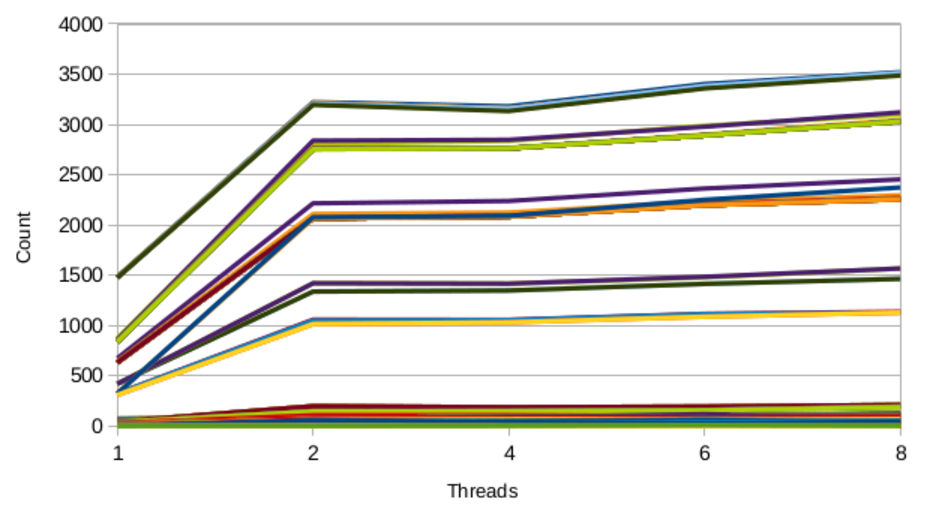
\includegraphics[width=0.4\textwidth]{images/cp2k-omp-inc-full.pdf}
\end{center}
\caption{Sampled reference counts to variables within OpenMP parallel regions}
\label{fig:openmp-refcount}
\end{figure}

\section{Conclusion and Future Work}
\label{sec:conclusion}
With this tool, we are able to gain new insight into applications and explore code and performance data in more ways and with a far finer level of detail than can be achieved with traditional analysis tools.
For administration, it can provide an easy and automated way of analysing usage patterns, and determining where to focus efforts on infrastructure and support.
Users can also benefit by using it to explore and analyse their code in a way that may have not been possible before, combining profiling data with structural data on the code to investigate things like memory and data structure usage patterns.

While there is already a very large degree of information this tool can provide and an unprecedented degree of flexibility, there are a still lot of directions this work could go, and a number of things necessary to help it get there.
One of the more notable such tasks is to actually reduce the level of information extracted down to more closely match what is actually utilised by end users as well as create a better and more language agnostic schema designed specifically with the tool in mind.
Both of these points result from the fact that the tool currently extracts internal C data structures within \acs{GCC} as is, which results in both a number of fields and storage methods for those fields as well as layout across data structures that may not always make quite as much sense for an \acs{SQL} database as it may for C code.
Additionally, once a mostly or entirely language agnostic schema is created, it can also pave the way toward easily dropping in support for C/C++ applications as well.
However, the best way to determine which fields are important and create such a schema, more and in-depth real world analysis of code is necessary in order to gain a better idea of what works and is needed.

Another future direction is to reinvestigate polyhedral analysis within the scope of this tool, and determine if and how it could be usefully applied to queries to enhance analysis.
Additionally, most of the queries we have constructed thus far have still remained confined within the scope of functions, so an alternative direction may be to explore more of an interprocedural analysis route.
Though this is well known for being a difficult problem to tackle, the level of detail and structure within this tool may provide some unique and unprecedented ways to perform such queries across function boundaries.

\section*{Acknowledgements}
\label{sec:ack}
% .25 pages
This work is supported by the United States \ac{DoE} and used resources of the \aclp{CRDP} and the \ac{OLCF} at \acl{ORNL}.

\bibliographystyle{splncs04}
\bibliography{references}
\end{document}
